\RequirePackage{currfile} 

\documentclass{beamer}

\usepackage{datetime}

% \usepackage[utf8]{inputenc}
\usepackage{amsmath}
% \usepackage{amsfonts}
% \usepackage{amssymb}
% \usepackage{datetime}
% \usepackage{float}
% \usepackage{graphicx}
\usepackage{url}
\usepackage[separate-uncertainty=true]{siunitx}
\usepackage{xcolor}

\usepackage{pgfplots}
\usepackage{pgfplotstable}
% \usepgfplotslibrary{groupplots}

\usepackage{booktabs} % for tables

\pgfplotsset{compat=newest}

% \usepackage[labelfont=bf,textfont=md, font=footnotesize]{caption}

% \usepackage[left=3.00cm, right=3.00cm, top=3.50cm, bottom=3.50cm]{geometry}


\usetheme{Boadilla}

\title[Parameter estimation]{Parameter estimation for the oscillating systems}

\author[Ashot Matevosyan, Aram Matevosyan]{
    Ashot Matevosyan\textsuperscript{1}, Aram Matevosyan\textsuperscript{2}
}
\institute[]{University of Cambridge\textsuperscript{1}, Yerevan State University\textsuperscript{2}}

\date[]{
Experiment performed \dayofweekname{18}{01}{2019} 18\textsuperscript{th} Januarty 2019
\newline
\newline
\today
}

\begin{document}

\begin{frame}
\titlepage
\end{frame}

\section{Apparatus and Methods}


\begin{frame}{Experiment details}
\framesubtitle{Apparatus}
\begin{figure}[t]
	\centering
	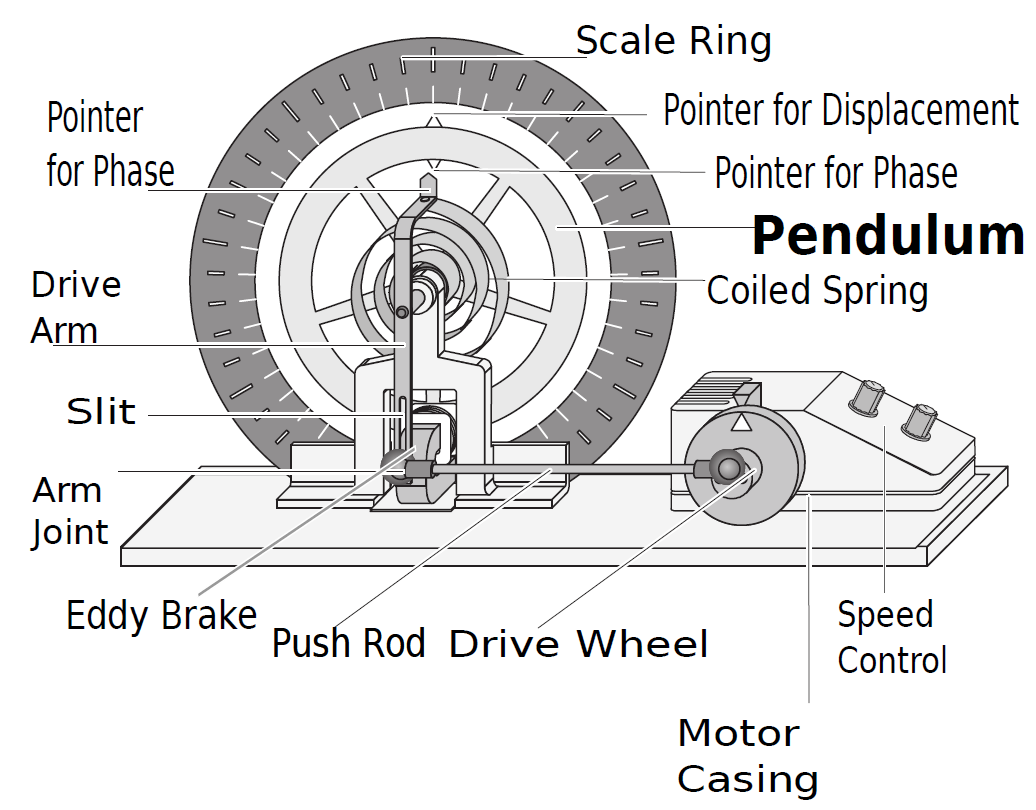
\includegraphics[width=0.7\linewidth]{images/pendulum_diagram.png}
	\caption{The diagram of the oscillating system in our experiment.}
	\label{fig:system-diagram}
\end{figure}
\end{frame}

\begin{frame}{Experiment details}
% \framesubtitle{Aparatus}
\begin{columns}
\column{0.6\textwidth}
\begin{itemize}
    \item<1-> Measure Amplitude by the ruler around the pendulum
    \item<2-> Measure period of oscillation by timer
    \item<3-> Measure and adjust frequency of the \textbf{driving force}
    \item<4-> Adjust \textbf{dumping force} by Eddy brake current
\end{itemize}
\column{0.4\textwidth}
\begin{figure}[t]
	\centering
	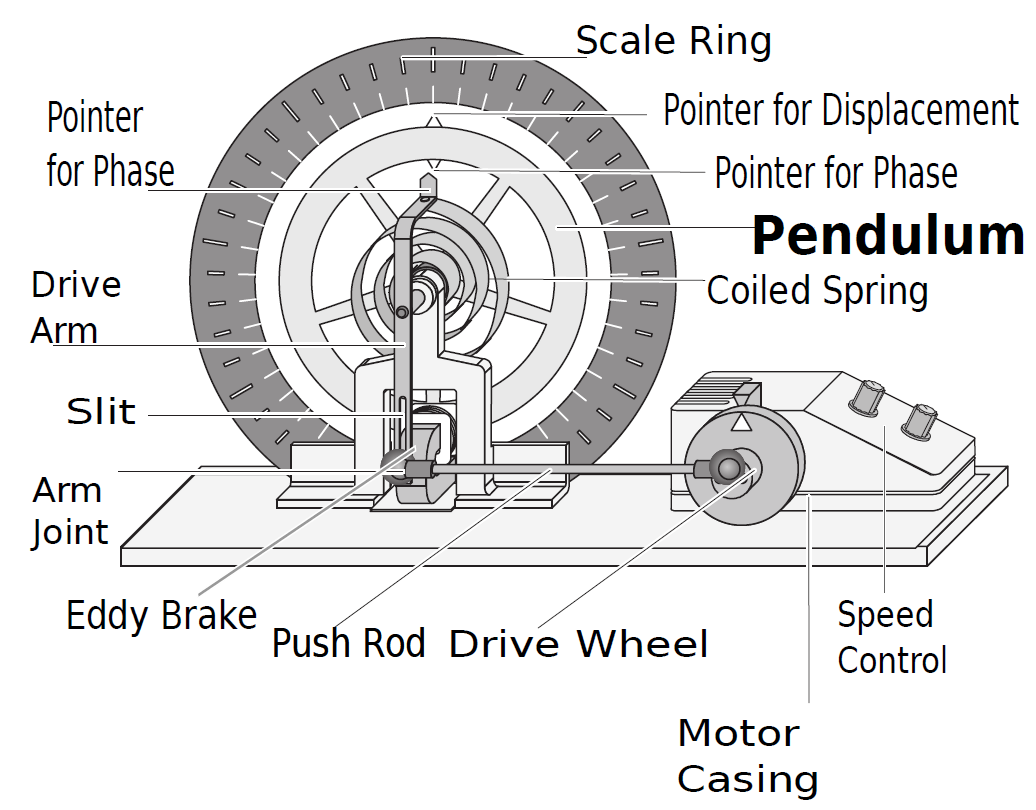
\includegraphics[width=1\linewidth]{images/pendulum_diagram.png}
	\label{fig:system-diagram}
\end{figure}
\end{columns}
\end{frame}

\section{Theoretical background}
\begin{frame}{Damped harmonic oscillator}
Equation of motion:
\begin{equation} \label{eq:motion-general}
	\ddot{\theta}+2 \gamma \dot{\theta} + \omega_0^2 \theta = 0
\end{equation}\begin{description}
\item[$\gamma$] measure of dumping
\item[$\omega_0$] natural frequency
\end{description}

\pause
Solution:
\begin{align}
	\begin{split}
	 \theta &= \theta_0 \, e^{-\gamma t} \cos(\omega_1 t) \\
	\text{where} \quad \omega_1 &=\sqrt{\omega_0^2-\gamma^2}
	\end{split}
\label{eq:motion-transient}
\end{align}
\end{frame}

\begin{frame}{Damped harmonic oscillator}
\begin{columns}
\column{0.33\textwidth}
\begin{figure}
	\centering
	\begin{tikzpicture}
	\begin{axis}[
	width=\linewidth*1.2,
	domain=0:4*pi,
	ymin=-1.5,ymax=1.5,
	%	axis lines=middle,
	axis x line=middle,
	axis y line=left,
	xtick=\empty,ytick=\empty,
	x label style={at={(axis description cs:0.5,+0.25)},anchor=north},
	]
	\addplot[black, samples=200]{exp(-x*0.3)* cos(deg(x*5))};	\addplot[black, dashed, samples=200]{exp(-x*0.3)};
	\addplot[black, dashed, samples=200]{-exp(-x*0.3)};
	\end{axis}
	\end{tikzpicture}
	\caption{Underdamped case, which has oscillatory motion.}
	\label{fig:underdamped}
\end{figure}
\column{0.33\textwidth}
\begin{figure}
	\begin{tikzpicture}
	\begin{axis}[
    width=1.2\linewidth,
	domain=0:4*pi,
	ymin=-1.5,ymax=1.5,
	%	axis lines=middle,
	axis x line=middle,
	axis y line=left,
	xtick=\empty,ytick=\empty,
	x label style={at={(axis description cs:0.5,+0.25)},anchor=north},
	]
	\addplot[black,dashed, samples=200]{exp(-x*2.5)*((2.5+2.37)*exp(+2.37*x) + (2.37-2.5)*exp(-2.37*x))/4.74};
	\addplot[black, samples=200]{exp(-0.8*x)*(1+0.8*x)};
	
	\end{axis}
	\end{tikzpicture}
	\caption{\textit{Critically damped} (solid), \textit{overdamped} (dashed) at the same natural frequency.}
	\label{fig:critical_over}
\end{figure}
\column{0.33\textwidth}
\begin{figure}\begin{tikzpicture}
		\begin{axis}[
		width=1.2\linewidth,
		domain=0:4*pi,
		ymin=-1.5,ymax=1.5,
		%	axis lines=middle,
		axis x line=middle,
		axis y line=left,
		x label style={at={(axis description cs:0.5,+0.25)},anchor=north},
		xtick=\empty,ytick=\empty,
		]
		\addplot[black,dashed, samples=200]{exp(-x*0.3)* cos(deg(x*2))};
		\addplot[black, samples=200]{exp(-0.3*x)*(1+0.3*x)};
		
		\end{axis}
		\end{tikzpicture}
		\caption{\textit{Critically damped} (dashed), \textit{underdamped} (doted) at the same damping constant.}
		\label{fig:critical_under}
\end{figure}
\end{columns}
\end{frame}

\begin{frame}{Quality factor}
\begin{definition}
    	\textit{Quality factor} is a dimensionless parameter that describes how underdamped the oscillator is, how well it oscillates. Quality factor Q is defined as
	\begin{equation}\label{eq:q-factor}
	Q=\cfrac{\omega_0}{2\gamma}
	\end{equation}
\end{definition}

\bigskip
For a \textit{good} oscillators $Q \gg 1$. 
\end{frame}

\begin{frame}{Forced oscillation}
Equation of motion:
\begin{equation} \label{eq:motion-general-forced}
	\ddot{\theta}+2 \gamma \dot{\theta} + \omega_0^2 \theta = f \, \cos(\omega t)
\end{equation}

\begin{description}
\item[$\gamma$] measure of dumping
\item[$\omega_0$] natural frequency
\item[$\omega$] angular frequency of the driving force
\item[$f$] measure of driving amplitude
\end{description}
\pause
Solution:
\begin{align}
\begin{split}
\theta(\omega) &=X(\omega)\cos(\omega t - \phi(\omega)) \\
X(\omega)&=\frac{f}{\sqrt{(\omega_0^2-\omega^2)^2+(2 \gamma \omega)^2}} \\
\tan \phi(\omega)&=\frac{2\gamma \omega}{\omega_0^2-\omega^2} \\
\end{split}
\end{align}
\end{frame}


\begin{frame}{Forced oscillation}
\begin{figure}[ht]
	\centering
	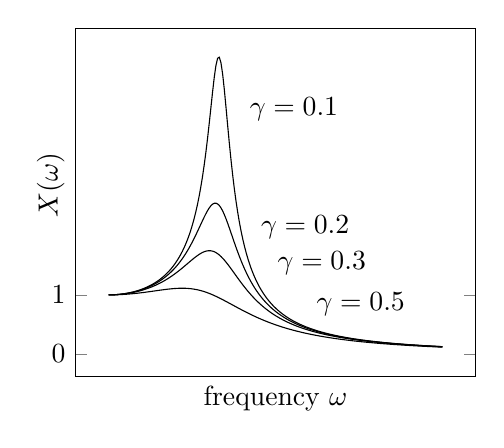
\begin{tikzpicture}[baseline]
	\begin{axis}[width=\textwidth*0.55,height=6cm,
	samples=200,domain=0:3,xlabel=frequency $\omega$, ylabel=$X(\omega)$,
	xtick=\empty,
	y label style={at={(axis description cs:-0.12,+0.55)},anchor=north},
	ytick={0,1}]
	\addplot[] {1/sqrt((1-x^2)^2+(2*x*0.1)^2)};
	\node at (axis cs:2.15,4.5) [anchor=north east] {$\gamma=0.1$};
	\addplot[] {1/sqrt((1-x^2)^2+(2*x*0.2)^2)};
	\node at (axis cs:2.25,2.5) [anchor=north east] {$\gamma=0.2$};
	\addplot[] {1/sqrt((1-x^2)^2+(2*x*0.3)^2)};
	\node at (axis cs:2.4,1.9) [anchor=north east] {$\gamma=0.3$};
	\addplot[] {1/sqrt((1-x^2)^2+(2*x*0.53)^2)};
	\node at (axis cs:2.75,1.2) [anchor=north east] {$\gamma=0.5$};
	\end{axis}
	\end{tikzpicture}%
	\hspace{0.2cm}
	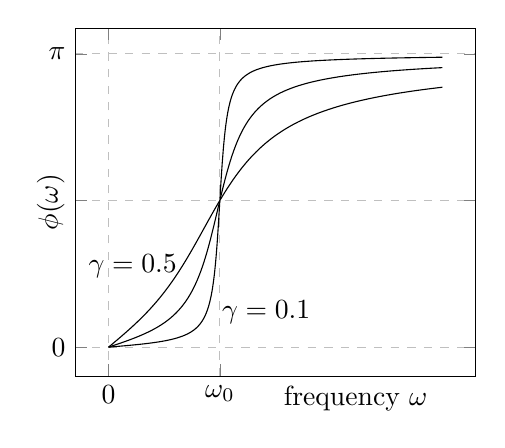
\begin{tikzpicture}[baseline]
	\begin{axis}[width=\textwidth*0.55,height=6cm,
	samples=200,domain=0:3,xlabel=frequency $\omega$, ylabel=$\phi(\omega)$,
	ytick={0,1.57, 3.14},
	yticklabels={$0$, \empty,$\pi$},
	xtick={0,1},
	xticklabels={$0$, $\omega_0$},
	x label style={at={(axis description cs:+0.7,-0.0)},anchor=north},
	y label style={at={(axis description cs:-0.12,+0.5)},anchor=north},
	grid style=dashed,
	xmajorgrids=true,ymajorgrids=true]
	\addplot[domain=0:1] {rad(atan(2*x*0.05/(1-x^2)))};
	\addplot[domain=1+0.001:3] {pi+rad(atan(2*x*0.05/(1-x^2)))};
	\node at (axis cs:1.9,0.6) [anchor=north east] {$\gamma=0.1$};
	\addplot[domain=0:1] {rad(atan(2*x*0.2/(1-x^2)))};
	\addplot[domain=1+0.001:3] {pi+rad(atan(2*x*0.2/(1-x^2)))};
	\addplot[domain=0:1] {rad(atan(2*x*0.5/(1-x^2)))};
	\addplot[domain=1+0.001:3] {pi+rad(atan(2*x*0.5/(1-x^2)))};
	\node at (axis cs:0.7,1.1) [anchor=north east] {$\gamma=0.5$};
	\end{axis}
	\end{tikzpicture}
	\caption{Dependence of \textit{amplitude} (on the left) and \textit{phase difference} (on the right) from frequency of the driving force}
	\label{fig:amplitude-frequency}
\end{figure}
\begin{columns}
\column{0.4\textwidth}
\begin{align*}
    \omega_{max} &= \sqrt{\omega_0^2-2\gamma^2}
\end{align*}
\column{0.6\textwidth}
\begin{align*}
    X_{max} \equiv X(\omega_{max}) &= \frac{f}{2\gamma\sqrt{\omega_0^2-\gamma^2}}
\end{align*}
\end{columns}

\end{frame}
\begin{frame}{Measurement of the Amplitude}
\begin{align*}
\onslide<1->{&\theta = \theta_0 \, e^{-\gamma t} \cos(\omega_1 t) \\}
\onslide<2->{\Rightarrow \; &a_n = a_0 \, e^{-n \gamma T} \text{  were  } T=\cfrac{2 \pi}{\omega_1} \\}
\onslide<3>{\Rightarrow \; &\ln(a_n) = ln(a_0) - n \gamma T }
\end{align*}
\end{frame}


\begin{frame}{Measurement of the Amplitude}
\framesubtitle{results}
\begin{figure}[ht]
	\centering	
	\begin{tikzpicture}
	\begin{axis}[
	legend pos=south east,
	width=0.9\linewidth,
	height=6cm,
	title={$ln(\text{amplitude})$ plotted as a function of the number of oscillations},
	xlabel={Number of oscillations, n},
	ylabel={$ln(\text{amplitude a\textsubscript{n} / arbitrary units})$ },
	xmajorgrids=true,ymajorgrids=true,
	grid style=dashed,
	]
	
	\addplot[
	color=blue,	only marks, mark=+,
	mark options={solid,scale=2,line width=0.5pt},
	error bars/.cd,
	y dir=both, y explicit,
	error bar style={line width=0.5pt,solid},
	error mark options={line width=0.7pt,mark size=3pt,rotate=90}
	]		
	table[x index = {0}, y index = {3}, y error plus index=4, y error minus index=5, col sep=comma]
	{data/transient_response_0.0A.csv};
	\addlegendentry{braking current = \SI{0.0}{\ampere}}
	
	\addplot [color=black,forget plot]
	table [col sep=comma, x index=0, 
	y={create col/linear regression={y=[index]3}}] 
	{data/transient_response_0.0A.csv};
	\xdef\slopeOne{\pgfplotstableregressiona}
	\xdef\interceptOne{\pgfplotstableregressionb}
	\node[] at (axis cs: 10,1.47){%
		$\pgfmathprintnumber{\slopeOne} \cdot x
		\pgfmathprintnumber[print sign]{\interceptOne}$};
	
	\addplot[color=orange, only marks, mark=+,
	mark options={solid,scale=2,line width=0.5pt},
	error bars/.cd,
	y dir=both, y explicit,
	error bar style={line width=0.5pt,solid},
	error mark options={line width=0.7pt,mark size=3pt,rotate=90}
	]		
	table[x index = {0}, y index = {3}, y error plus index=4, y error minus index=5, col sep=comma]
	{data/transient_response_0.6A.csv};
	\addlegendentry{braking current = \SI{0.6}{\ampere}}
	
	\addplot [color=black]
	table [col sep=comma, x index=0, 
	y={create col/linear regression={y=[index]3}}] 
	{data/transient_response_0.6A.csv};
	\xdef\slopeTwo{\pgfplotstableregressiona}
	\xdef\interceptTwo{\pgfplotstableregressionb}
	\node[] at (axis cs: 6.7,-0.0){%
		$\pgfmathprintnumber[precision=3]{\slopeTwo} \cdot x
		\pgfmathprintnumber[print sign]{\interceptTwo}$};
	
	\end{axis}
	\end{tikzpicture}
	\caption{$\ln(\text{amplitude})$ versus oscillation number $n$. Dependence is linear as we expected.}
	\label{fig:log-plot}
	\end{figure}

\end{frame}

\begin{frame}{Results}
\begin{align*}
\ln(a_n) = ln(a_0) - n \gamma T \\
\text{slope of the line} =  -\gamma \, T = -\gamma \cfrac{2 \pi}{\omega_1}
\end{align*}
\pause

For low damping $\omega_1 \approx \omega_0$ so the slope is approximately $-\cfrac{\pi}{Q}$.
\begin{table}\centering
\begin{tabular}{c c} 
	\toprule
	slope [$I_b=0.0A]$ & \num{-0.044 \pm 0.001}\\
	slope [$I_b=0.6A]$ & \num{-0.80 \pm 0.03} \\
	\bottomrule
\end{tabular}
\end{table}
\pause
And by assumption $\text{slope} \approx -\cfrac{\pi}{Q}$
\begin{table}[H]\centering
	\begin{tabular}{c c} 
		\toprule
		Q [$I_b=0.0A$] & \num{71 \pm 1} \\
		Q [$I_b=0.6A$] & \num{3.9 \pm 0.1} \\
		\bottomrule
	\end{tabular}
\end{table}

\end{frame}


\begin{frame}{Forced oscillation}
\framesubtitle{Resonance curve}
\begin{figure}[ht]
   		\begin{tikzpicture}
   		\begin{axis}[
   		width=\linewidth,height=7cm,
   		title={Amplitude of forced oscillations as a function of angular frequency},
   		xlabel={Angular frequency / $s^{-1}$},
   		ylabel={Amplitude / arbitrary units},
   		xmajorgrids=true,ymajorgrids=true,
   		grid style=dashed,
   		]
   		
   		\addplot[smooth, solid,	color=blue,	mark=+,
   		mark options={solid,scale=2,line width=1.5pt}]		
   		table[x index = {3}, y index = {6}, col sep=comma]
   		{data/forced_oscillations_0.3A.csv};
   		\addlegendentry{braking current = \SI{0.3}{\ampere}}
   		\addplot [color=green,opacity=0.4, mark=*, mark size=5pt, forget plot] 
   		coordinates {(3.11,11.5)};
   		\draw [dashed,thick, color=black] (axis cs: -10,11.5) -| (axis cs: 3.11,-10);
   		
   		
   		\addplot[smooth, solid,	color=orange,	mark=+,
   		mark options={solid,scale=2,line width=1.5pt},
   		]		
   		table[x index = {3}, y index = {6}, col sep=comma]
   		{data/forced_oscillations_0.6A.csv};
   		\addlegendentry{braking current = \SI{0.6}{\ampere}}
   		\addplot [color=green,opacity=0.4, mark=*, mark size=5pt, forget plot] 
   		coordinates {(3.05,3.3)};
   		\draw [dashed,thick, color=black] (axis cs: -10,3.3) -| (axis cs: 3.05,-10);
   		
   		\end{axis}
   		\end{tikzpicture}
   		\label{fig:resonance-curve}
   	\end{figure}
\end{frame}

\begin{frame}{Forced oscillation}
\framesubtitle{Analysis}
\begin{equation}\label{eq:solution-amplitude}
	X(\omega)=\frac{f}{\sqrt{(\omega_0^2-\omega^2)^2+(2 \gamma \omega)^2}} \quad \Rightarrow \quad X(0) = \frac{f}{\omega_0}
\end{equation}
\pause
\begin{align}
\begin{split}
X_{max} = \frac{f}{2\gamma\sqrt{\omega_0^2-\gamma^2}}
\end{split}
\label{eq:solution-omega-max}
\end{align}
\pause
When $\gamma \ll \omega_0$
\begin{align}
\begin{split}
X_{max} \approx \frac{f}{2\gamma\omega_0} &= \frac{f}{\omega_0^2} \cdot \frac{\omega_0}{2\gamma}\\
&=X(0) \cdot Q
\end{split}
\label{eq:alt-q-factor}
\end{align}
\end{frame}


\begin{frame}{Forced oscillation}
\framesubtitle{Amplitude at zero frequency}
To measure the amplitude at $\omega=0$ the drive wheel was rotated  slowly by hand and the maximum displacement of the pendulum on either side of zero was read.
   
\begin{figure}[t]
\centering
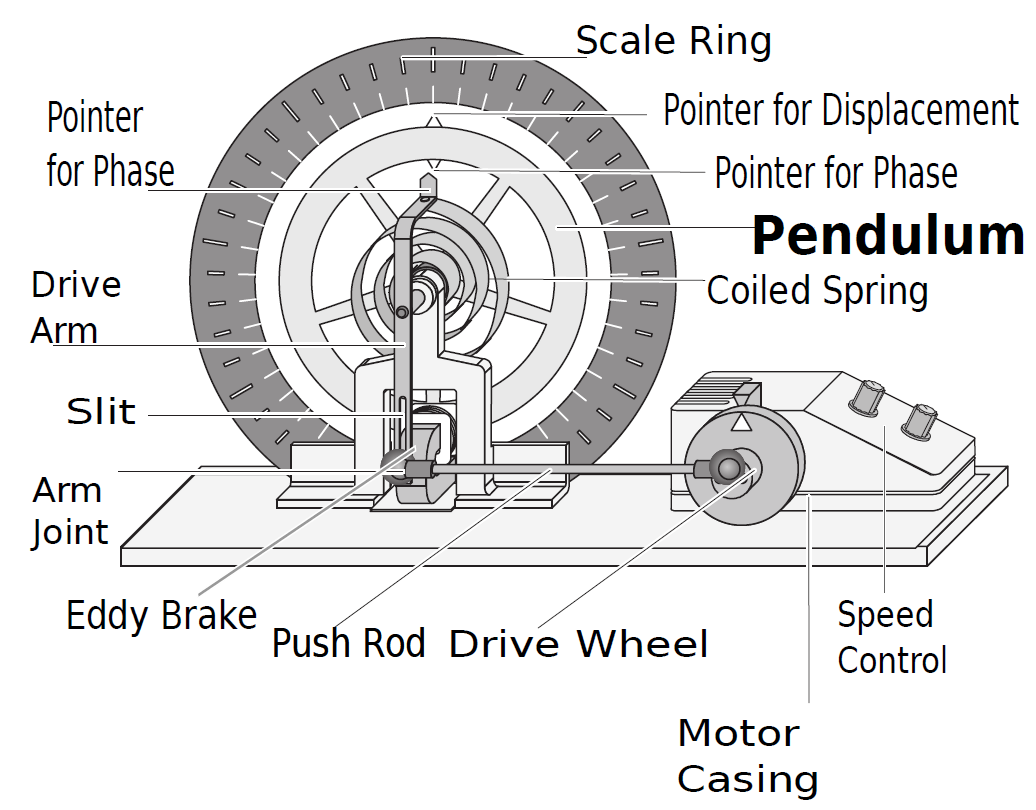
\includegraphics[width=0.5\linewidth]{images/pendulum_diagram.png}
\label{fig:system-diagram}
\end{figure}
Amplitude at $\omega = 0$ estimated to be $X(0) = \num{0.7 \pm 0.1}$.
\end{frame}



\begin{frame}{Forced oscillation}
\framesubtitle{Results}
Resonance frequency and the amplitude at resonance from the plot.
\begin{table}
   \centering
   \begin{tabular}{c c c}
   	\toprule
   	& $X_{max}$ & $\omega_{max} $\\
   	\midrule
   	$I_b=\num{0.3}\si{\ampere}$ & \num{11.5 \pm 0.1} & \num{3.11 \pm 0.02} \si{\per\second}\\
   	$I_b=\num{0.6}\si{\ampere}$ & \num{3.3 \pm 0.1} & \num{3.05 \pm 0.05} \si{\per\second}\\
   	\bottomrule
   \end{tabular}
   \label{table:resonance-results}
\end{table}
Thus, Quality factors are estimated to be:
   \begin{table}[H]\centering
   	\begin{tabular}{c c} 
   		\toprule
   		$Q^{2nd}$ [$I_b=0.3A$] & \num{16 \pm 2} \\
   		$Q^{2nd}$ [$I_b=0.6A$] & \num{4.7 \pm 0.7} \\
   		\bottomrule
   	\end{tabular}
   \end{table}
\end{frame}
\begin{frame}{Mean and std estimation}
\framesubtitle{Problem setup}


\begin{problem}
Given i.i.d. samples from \textit{Normal distribution}:
\begin{equation*}
x_i \overset{\text{iid}}{\sim} \mathcal{N}(\,\, \cdot \,\, | \, \mu, \sigma^2) \text{\quad  for i=1,2,3 ..., N}
\end{equation*}
Suppose $\sigma$ is known. Find estimation for $\mu$.
\end{problem}
\pause
\begin{solution}
\begin{equation*}
    \hat{\mu} = \frac{1}{N} \sum_{i=0}^N{x_i} \quad \text{(Sample mean)}
\end{equation*}
\end{solution}
\pause
\textbf{This solution does not satisfy!}

Sometimes we need to know \textbf{uncertainty} in our measurements.
How much confident are we in out estimation?
\end{frame}

\begin{frame}{Bayesian Inference}
\framesubtitle{Introduction}
\begin{theorem}[Bayes' Theorem]
\begin{equation*}
P(A \mid B) = \frac{P(B \mid A) \, P(A)}{P(B)}
\end{equation*}
\end{theorem}
\pause
\begin{example}
We are given \textbf{Data}, we want to find \textbf{distribution over parameters}:
\begin{equation*}
    P( Parametes \mid Data ) = \frac{P( Data \mid Parameters ) \, P(Parameters)}{P(Data)}
\end{equation*}
\end{example}
\pause
\begin{description}[leftmargin=1cm, labelwidth=3cm]
\item[$P(Parameters)$] Prior
\item[$P( Parametes \mid Data ) $] Posterior
\item[$P( Data \mid Parameters )$] Likelihood
\item[$P(Data)$] Marginal
\end{description}
\end{frame}

\begin{frame}{Bayesian Inference}
\framesubtitle{Introduction}
\begin{theorem}[Bayes' Theorem]
\begin{equation*}
P(A \mid B) = \frac{P(B \mid A) \, P(A)}{P(B)}
\end{equation*}
\end{theorem}

\begin{example}
We are given \textbf{Data}, we want to find \textbf{distribution over parameters}:
\begin{equation*}
    P( \mu \mid \{x_i\} ) = \frac{P( \{x_i\} \mid \mu ) \, P(\mu)}{P(\{x_i\})}
\end{equation*}
\end{example}

\begin{description}[leftmargin=1cm, labelwidth=3cm]
\item[$P(\mu)$] Prior
\item[$P( \mu \mid \{x_i\} ) $] Posterior
\item[$P( \{x_i\} \mid \mu )$] Likelihood
\item[$P(\{x_i\})$] Marginal
\end{description}
\end{frame}




\begin{frame}{Modeling The Problem}
\framesubtitle{Likelihood}
Likelihood for each sample is
\begin{equation*}
    p\left(x_{i} \mid \mu\right)=\left(2 \pi \sigma^{2}\right)^{-1 / 2} \exp \left(-\frac{1}{2} \frac{\left(x_{i}-\mu\right)^{2}}{\sigma^{2}}\right)
\end{equation*}
\pause
and as samples are i.i.d., the \textit{Likelihood of the Data} is
\pause
\begin{equation*}
    p(x \mid \mu)=\prod_{i=1}^{n} p\left(x_{i} \mid \mu\right)=\left(2 \pi \sigma^{2}\right)^{-n / 2} \exp \left(-\frac{1}{2 \sigma^{2}} \sum_{i=1}^{n}\left(x_{i}-\mu\right)^{2}\right)
\end{equation*}
    
\end{frame}

\begin{frame}{Modeling The Problem}
\framesubtitle{Prior and Marginal}
\textbf{Prior} (belief) for $\mu$ we take
\begin{equation*}
    p(\mu)=\mathcal{N}\left(\mu | \mu_{0}, \sigma_{0}^{2}\right)
\end{equation*}
\pause
And so, \textbf{Marginal} will be
\begin{equation*}
    p(x) = \int_{-\infty}^{\infty}p(x \mid \mu) p(\mu) d\mu    
\end{equation*}
\pause
Note that this is the hardest part of the model. Sometimes his integral could be intractable. \\
Also note that this is normalisation constant and
\begin{equation*}
    p(\mu \mid x) \sim p(x \mid \mu) p(\mu)
\end{equation*}
\end{frame}

\begin{frame}{Sample Mean estimation}
\begin{problem}
\begin{equation*}
x_i \overset{\text{iid}}{\sim} \mathcal{N}(\,\, \cdot \,\, | \, \mu, \sigma^2) \text{\quad  for i=1,2,3...,N}. \text{ Find estimation for }\mu.
\end{equation*}
\end{problem}
\pause
\begin{solution}[Maximum likelihood]
\begin{equation*}
    \hat{\mu}_{\mathrm{ML}} = \frac{1}{N} \sum_{i=0}^N{x_i} \quad \text{(Sample mean)}
\end{equation*}
\end{solution}
\pause

\begin{solution}[Bayesian  inference~\footnotemark ]
\begin{gather*}
p(\mu \mid x)=\mathcal{N}\left(\mu \mid \mu_{N}, \sigma_{N}^{2}\right) \\
\text{ where } \quad  \mu_{N} =\frac{\sigma^{2}}{N \, \sigma_{0}^{2}+\sigma^{2}} \mu_{0}+\frac{N \, \sigma_{0}^{2}}{N \, \sigma_{0}^{2}+\sigma^{2}} \mu_{\mathrm{ML}} \ \text{ and } \  \frac{1}{\sigma_{N}^{2}} =\frac{1}{\sigma_{0}^{2}}+\frac{N}{\sigma^{2}} 
\end{gather*}
\end{solution}

\alt<2>{\let\thefootnote\relax\footnotetext{~}}{\footnotetext{Christopher M. Bishop, \textit{Pattern Recognition and Machine Learning}, Chapter 2.3.6}}

\end{frame}

\begin{frame}{Model for oscillating system}
From our experiment we have $(\omega_i, X_i)$ $i=1,...,N$ pairs, where $N$ is number of measurements. We can \textit{assume} that our measurements come from distribution
  \begin{equation*}\label{eq:distribution}
  X_i \, \overset{\text{iid}}{\sim} \,  
  \mathcal{P}(\,\, \cdot \,\, | \, \omega_i, \omega_0, X_0, \gamma) \equiv \mathcal{N}(X(\omega_i; \, \omega_0, X_0, \gamma),\,\sigma^{2})\ \quad 
  \text{   for   } i=1,...,n
  \end{equation*}
  \begin{equation*}\label{eq:solution-amplitude-new}
  \text{where} \ X(\omega; \, \omega_0, X_0, \gamma) = \frac{X_0 \, \omega_0^2} {\sqrt{(\omega_0^2-\omega^2)^2+(2 \gamma \omega)^2}}
  \end{equation*}
  \pause
  As precision of our measurements is 0.1, we take $\sigma = 0.1$.
  
  Our task is to estimate parameters $\omega_0,\, \gamma$ and $X_0$ from the resonance curve $(\omega_i, X_i)_{1...n}$. More formally, find \textbf{posterior distribution}
  \begin{equation}\label{eq:inference1}
  \omega_0, \, \gamma, \, X_0 \sim \mathcal{P}(\,\, \cdot \,\, | \, \omega_1...\omega_n, X_1...X_n)
  \end{equation}
\end{frame}

\begin{frame}{Using Bayes' Theorem}
For Posterior distribution we have
\begin{align*}
  \begin{split}
  \mathcal{P}(\omega_0, \gamma,X_0\,|\,X_1...X_n, \omega_1...\omega_n) &=
  \cfrac{\mathcal{P}(X_1...X_n\,|\,\omega_0,\gamma,X_0,\omega_1...\omega_n) \cdot
  	\mathcal{P}(\omega_0,\gamma,X_0)
  }{\textit{margnal}} \\
\textcolor{green}{\text{i.i.d assumption} \ }&= \cfrac{\prod\limits_{i=1}^{n}\mathcal{P}(X_i\,|\,\omega_0,\gamma,X_0, \omega_i) \cdot
	\mathcal{P}(\omega_0,\gamma,X_0)
}{\textit{margnal}}
\end{split}
\end{align*}
\pause
We take \textit{Gamma distributions} for priors of $\omega_0$, $\gamma$ and $X_0$. 

\begin{figure}
	\centering
	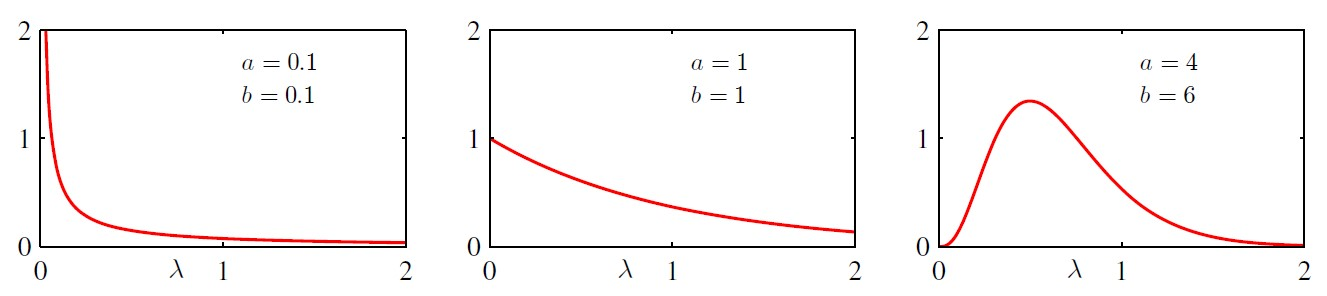
\includegraphics[width=\linewidth]{images/gamma.jpg}
	\caption{Gamma distribution pdf for different parameter values.}
\end{figure}
\end{frame}

\begin{frame}{Method}
Unfortunately we can't get analytical form of the \textit{Posterior}. But we do not need analytical form anyway. \textbf{Samples from Posterior distribution are enough!}
\\~\\
\pause
There are different sampling algorithms and frameworks. We have used \textbf{Stan}\footnotemark which uses \textit{Markov chain Monte Carlo} (MCMC) sampling algorithm.
\\~\\
\pause
Now we sample from our posterior distribution. Our samples are triplets ($\omega_0$, $\gamma$,$X_0$)\textsubscript{$i$}. \\
\textbf{Sample mean} and \textbf{sample std} for each parameter are \textbf{estimation} and \textbf{uncertainty} for that parameter respectively.

\alt<2>{\let\thefootnote\relax\footnotetext{~}}{\footnotetext{Stan statistical modeling platform \ \href{https://mc-stan.org/}{\url{https://mc-stan.org/}}}}

\end{frame}

\begin{frame}{Results}
\begin{onlyenv}<1-5>
\begin{figure}[h]
    \makebox[\textwidth][c]{%
	\includegraphics<1>[width=1.2\textwidth]{images/samples_003.png}
	\includegraphics<2>[width=1.2\textwidth]{images/samples_010.png}
	\includegraphics<3>[width=1.2\textwidth]{images/samples_030.png}
	\includegraphics<4>[width=1.2\textwidth]{images/samples_100.png}
	\includegraphics<5>[width=1.2\textwidth]{images/samples_err.png}
	}
\end{figure}
\end{onlyenv}
\end{frame}


\begin{frame}{Results}
\vspace{0.3cm}
\begin{columns}
\column{0.5\textwidth}
\Large \centering Braking current $=0.3\si{\ampere}$
\begin{figure}[t]
	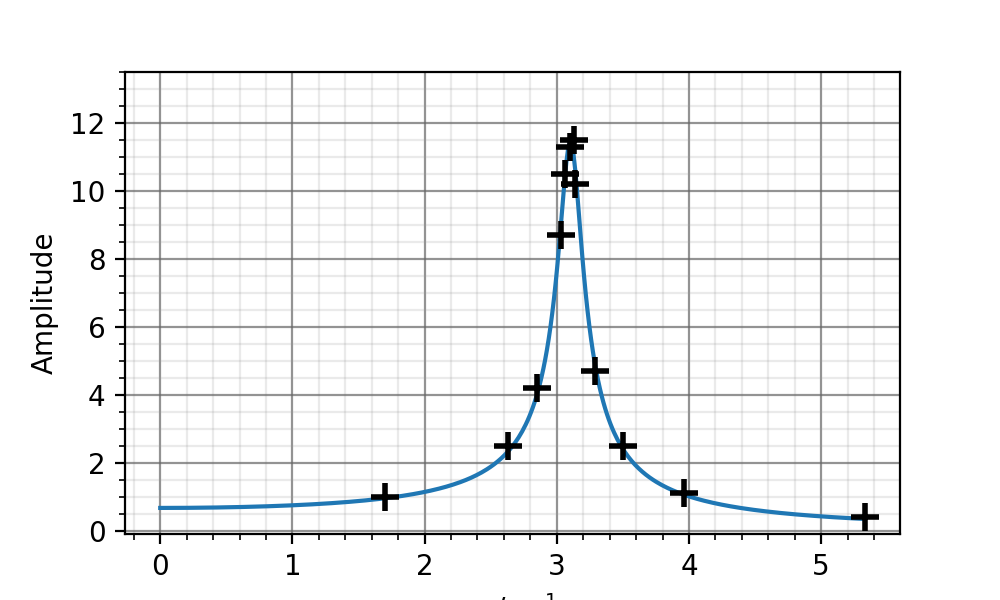
\includegraphics[width=0.95\linewidth]{images/result03.png}
\end{figure}
\column{0.5\textwidth}
\Large \centering Braking current $=0.6\si{\ampere}$
\begin{figure}[t]
	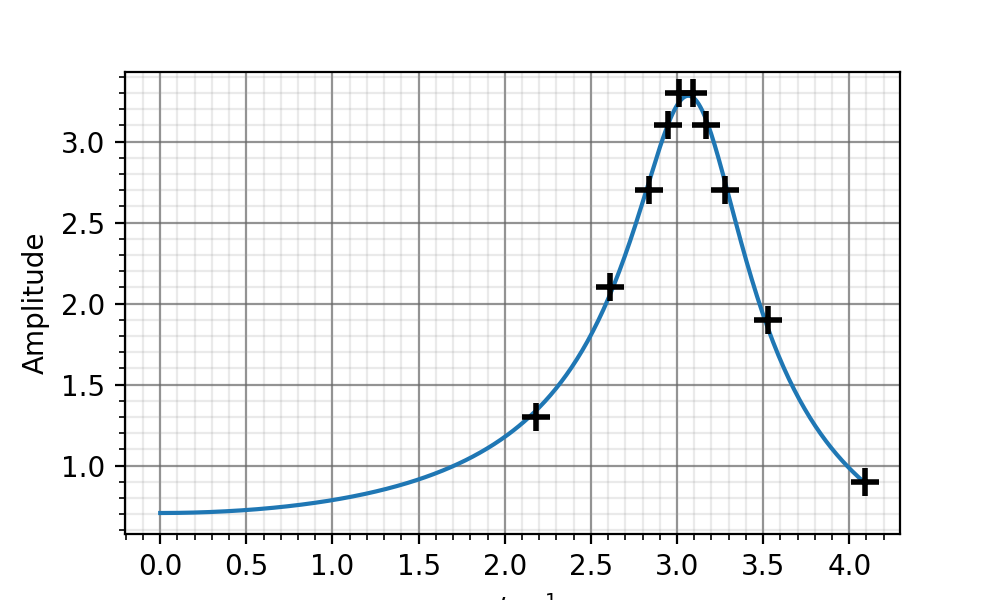
\includegraphics[width=0.95\linewidth]{images/result06.png}
\end{figure}
\end{columns}
\pause
  \begin{table}[ht]
  	\centering
  	\begin{tabular}{c c c}
  		\toprule
  		& $I_b=0.3\, \si{\ampere}$ & $I_b=0.6 \, \si{\ampere} $\\
  		\midrule
  		$\omega_0$ / \si{\per\second} & \num{3.10584 \pm 0.00012} & \num{3.1025 \pm 0.0013} \\
  		$\gamma$ / \si{\per\second} & \num{0.09059 \pm 0.00016} & \num{0.3363 \pm 0.0018} \\
  		$X_0 \equiv X(0)$ & \num{0.6675 \pm 0.0010} & \num{0.708 \pm 0.003} \\
  		$Q^{3th}$ / \si{\per\second} & \num{17.14 \pm 0.03} & \num{4.61 \pm 0.02} \\
  		\bottomrule
  	\end{tabular}
  	\caption{Resonance frequency and the amplitude at resonance.}
  	\label{table:resonance-infered-results}
  \end{table}
  
  
\end{frame}

\end{document}
